% Use this template to write your solutions to COS 423 problem sets

\documentclass[12pt]{article}
\usepackage[utf8]{inputenc}
\usepackage{amsmath, amsfonts, amsthm, amssymb, algorithm, graphicx, mathtools,xfrac}
\usepackage[noend]{algpseudocode}
\usepackage{fancyhdr, lastpage}
\usepackage[vmargin=1.20in,hmargin=1.25in,centering,letterpaper]{geometry}
\setlength{\headsep}{.50in}
\setlength{\headheight}{15pt}

% Landau notation
\DeclareMathOperator{\BigOm}{\mathcal{O}}
\newcommand{\BigOh}[1]{\BigOm\left({#1}\right)}
\DeclareMathOperator{\BigTm}{\Theta}
\newcommand{\BigTheta}[1]{\BigTm\left({#1}\right)}
\DeclareMathOperator{\BigWm}{\Omega}
\newcommand{\BigOmega}[1]{\BigWm\left({#1}\right)}
\DeclareMathOperator{\LittleOm}{\mathrm{o}}
\newcommand{\LittleOh}[1]{\LittleOm\left({#1}\right)}
\DeclareMathOperator{\LittleWm}{\omega}
\newcommand{\LittleOmega}[1]{\LittleWm\left({#1}\right)}

% argmin and argmax
\newcommand{\argmin}{\operatornamewithlimits{argmin}}
\newcommand{\argmax}{\operatornamewithlimits{argmax}}

\newcommand{\calP}{\mathcal{P}}
\newcommand{\Z}{\mathbb{Z}}
\newcommand{\R}{\mathbb{R}}
\newcommand{\Exp}{\mathbb{E}}
\newcommand{\Q}{\mathbb{Q}}
\newcommand{\sign}{\mathrm{sign\ }}
\newcommand{\abs}{\mathrm{abs\ }}
\newcommand{\eps}{\varepsilon}
\newcommand{\zo}{\{0, 1\}}
\newcommand{\SAT}{\mathit{SAT}}
\renewcommand{\P}{\mathbf{P}}
\newcommand{\NP}{\mathbf{NP}}
\newcommand{\coNP}{\co{NP}}
\newcommand{\co}[1]{\mathbf{co#1}}
\renewcommand{\Pr}{\mathop{\mathrm{Pr}}}

% theorems, lemmas, invariants, etc.
\newtheorem{theorem}{Theorem}
\newtheorem{lemma}[theorem]{Lemma}
\newtheorem{invariant}[theorem]{Invariant}
\newtheorem{corollary}[theorem]{Corollary}
\newtheorem{definition}[theorem]{Definition}
\newtheorem{property}[theorem]{Property}
\newtheorem{proposition}[theorem]{Proposition}

% piecewise functions
\newenvironment{piecewise}{\left\{\begin{array}{l@{,\ }l}}
{\end{array}\right.}

% paired delimiters
\DeclarePairedDelimiter{\ceil}{\lceil}{\rceil}
\DeclarePairedDelimiter{\floor}{\lfloor}{\rfloor}
\DeclarePairedDelimiter{\len}{|}{|}
\DeclarePairedDelimiter{\set}{\{}{\}}

\makeatletter
\@addtoreset{equation}{section}
\makeatother
\renewcommand{\theequation}{\arabic{section}.\arabic{equation}}

% algorithms
\algnewcommand\algorithmicinput{\textbf{INPUT:}}
\algnewcommand\INPUT{\item[\algorithmicinput]}
\algnewcommand\algorithmicoutput{\textbf{OUTPUT:}}
\algnewcommand\OUTPUT{\item[\algorithmicoutput]}


% Formating Macros

\pagestyle{fancy}
\lhead{\sc \hmwkClass $\;\;\cdot \;\;$ \hmwkSemester $\;\;\cdot\;\;$
Problem \hmwkAssignmentNum.\hmwkProblemNum}
%\chead{\sc Problem \hmwkAssignmentNum.\hmwkProblemNum}
%\chead{}
\rhead{\em \hmwkAuthorName\ $($\hmwkAuthorID$)$}
\cfoot{}
\lfoot{}
\rfoot{\sc Page\ \thepage\ of\ \protect\pageref{LastPage}}
\renewcommand\headrulewidth{0.4pt}
\renewcommand\footrulewidth {0.4pt}

\fancypagestyle{fancycollab}
{
    \lfoot{\em Collaborators: \hmwkCollaborators}
}

\fancypagestyle{problemstatement}
{
    \rhead{}
    \lfoot{}
}

%%%%%% Begin document with header and title %%%%%%%%%%%%%%%%%%%%%%%%%

\begin{document}

%%%%%% Header Information %%%%%%%%%%%%%%%%%%%%%%%%%%%%%%%%%%%%%%%%%%%

%%% Shouldn't need to change these
\newcommand{\hmwkClass}{CS 255}
\newcommand{\hmwkSemester}{Spring 2016}

%%% Your name, in standard First Last format
\newcommand{\hmwkAuthorName}{Christian Rentsman}
%%% Your NetID
\newcommand{\hmwkAuthorID}{crentsman}

%%% The problem set number (just the number)
\newcommand{\hmwkAssignmentNum}{5}

%%% The problem number (just the number)
\newcommand{\hmwkProblemNum}{1}

%%% A list of your collaborators' NetIDs, separated by ", ".
%%% You can use a new line ("\\") in the middle to prevent a long
%%% list from overflowing.
\newcommand{\hmwkCollaborators}{}
%%% Sets the collaborator list to appear on the first page
\thispagestyle{fancycollab}

%%%%%%% begin Solution %%%%%%%%%%%%%%%%%%%%%%%%%%%%%%%%%%%%%%%%%%%%%

\section{Problem C: Catering}

\subsection{Problem Specification}


Paul owns a catering company and business is booming. The company has $k$
catering teams, each in charge of one set of catering equipment. Every
week, the company accepts $n$ catering requests for various events.
For every request, they send a catering team with their equipment to the
event location. The team delivers the food, sets up the equipment, and instructs
the host on how to use the equipment and serve the food. After the event, the
host is responsible for returning the equipment back to Paul’s company.

Unfortunately, in some weeks the number of catering teams is less than the number
of requests, so some teams may have to be used for more than one event. In these
cases, the company cannot wait for the host to return the equipment and must keep
the team on-site to move the equipment to another location. The company has an
accurate estimate of the cost to move a set of equipment from any location to any
other location. Given these costs, Paul wants to prepare an Advance Catering Map
to service the requests while minimizing the total moving cost of equipment
(including the cost of the first move), even if that means not using all the
available teams. Paul needs your help to write a program to accomplish this task.
The requests are sorted in ascending order of their event times and they are
chosen in such a way that for any $i < j$, there is enough time to
transport the equipment used in the $i$-th request to the location of the
$j$-th request.

\subsection{Mathematical Formulation}

\subsection{Problem Size}

We are given an unknown amount of test cases that we have to solve in under
three seconds. However, our given variables do have bounds. The number
of teams, $k$, and the number of requests, $n$, are both bounded by
0 and 100, inclusive. The $i$th request (counting from 1) has $n - i + 1$
connections to the requests after it.

\subsection{Solution Description}

To solve this problem, we model the input as a bipartite graph, and
then try to find a minimum cost matching. Therefore, the main parts
of our algorithm are: read in the input and build an adjacency matrix
for a bipartite graph, and then, using that graph and a minimum
cost bipartite matching algorithm with Dijkstra's single source
shortest paths (with an indexed minimum priority queue), find the
minimum cost matching.

The main runner for our program is written below. It is essentially
the algorithm described above.

\begin{algorithm}[H]
\caption{Main runner of our program.}
\begin{algorithmic}
    \Procedure{Main}{}
        \State $in \gets$ new Scanner for system.in
        \While{$in$ has more integers to read}
            \State $n \gets$ next integer from $in$
            \State $k \gets$ next integer from $in$
            \State $g \gets$ \Call{BuildGraphFromInput}{$in, n, k$}
            \State $minCost \gets$ \Call{GetMinCostMatching}{$g, n, k$}
            \State \Call{Print}{$minCost$}
        \EndWhile
    \EndProcedure
\end{algorithmic}
\end{algorithm}

Before we can even solve the problem, we have to build a graph which
represents it. When we call the {\sc BuildGraphFromInput} method,
we read in the input from standard input and we build our bipartite
graph using that data. The algorithm for building the graph is
detailed below:

\begin{algorithm}[H]
\caption{Builds a bipartite graph from the input.}
\begin{algorithmic}
    \Procedure{BuildGraphFromInput}{$in, n, k$}
        \State $numNodes \gets 1 + k + (2 \times n)$
        \State $leftStart \gets 1$
        \State $rightStart \gets k + n$
        \State $g \gets$ new array of size ($numNodes \times numNodes$)
        \State Fill up all indices of $g$ with $\infty$
        \State $teamValues \gets$ new array of size ($numNodes$)
        \\
        \For{$i \in [0, numNodes)$}
            \State $teamValues[i] \gets$ next integer from $in$
        \EndFor
        \For{$u \in [leftStart, k]$}
            \For{$i \in [0, n)$}
                \State $g[u][k + n + i] \gets teamValues[i]$
            \EndFor
        \EndFor
        \For{$u \in [leftStart + k, rightStart)$}
            \For{$v \in [u + n, numNodes - 1)$}
                \State $g[u][v] \gets$ next integer from $in$
            \EndFor
        \EndFor
        \For{$i \in [leftStart, rightStart)$}
            \State $g[0][i] \gets 0$
        \EndFor
        \For{$i \in [rightStart, numNodes - 1)$}
            \State $g[i][numNodes - 1] \gets 0$
        \EndFor
        \\
        \State \Return $g$
    \EndProcedure
\end{algorithmic}
\end{algorithm}

After building our bipartite graph, we simply run a minimum cost
bipartite matching algorithm (our specific implementation utilizes
Dijkstra's Single Source Shortest Paths algorithm with an indexed
minimum priority queue) to find the minimum matching cost. This is
done within the {\sc GetMinCostMatching} method. After doing that,
we just print out the value we found and, thus, the problem is solved.

\subsection{Examples and Test Cases}

To show how our algorithm actually works, we'll run through a quick
example using one of the sample test cases. Say our input is as
follows:

\begin{center}
    3 2 \\
    40 30 40 \\
    50 10 \\
    50
\end{center}

This means that we have three requests ($n = 3$) and two teams ($k = 2$).
We can draw this input as a location graph, showing us the connections
between different locations and the costs to move from one location
to another.

\begin{center}
    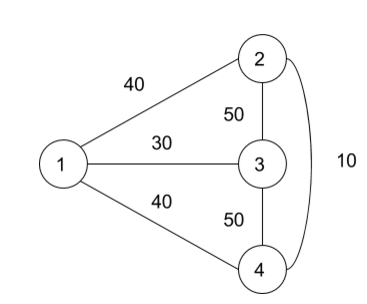
\includegraphics[scale=0.5]{catering1}
\end{center}

However, to actually solve this problem, we need to create a bipartite
graph so we can use the minimum cost bipartite matching algorithm. The
graph and the corresponding adjacency matrix can be found below (vertex
numbers are in parentheses, T means team, and L means location):

\begin{center}
    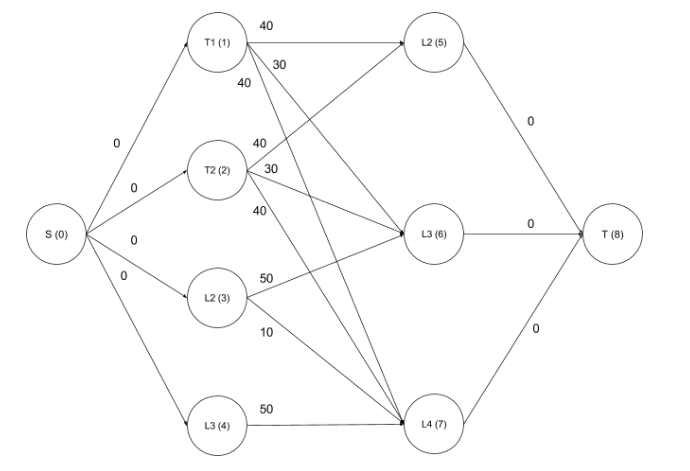
\includegraphics[scale=0.5]{catering_example_graph}
\end{center}

\begin{center}
    \[
        \begin{bmatrix}
            \infty & 0 & 0 & 0 & 0 & \infty & \infty & \infty & \infty \\
            \infty & \infty & \infty & \infty & \infty & 40 & 30 & 40 & \infty \\
            \infty & \infty & \infty & \infty & \infty & 40 & 30 & 40 & \infty \\
            \infty & \infty & \infty & \infty & \infty & \infty & 50 & 10 & \infty \\
            \infty & \infty & \infty & \infty & \infty & \infty & \infty & 50 & \infty \\
            \infty & \infty & \infty & \infty & \infty & \infty & \infty & \infty & 0 \\
            \infty & \infty & \infty & \infty & \infty & \infty & \infty & \infty & 0 \\
            \infty & \infty & \infty & \infty & \infty & \infty & \infty & \infty & 0 \\
            \infty & \infty & \infty & \infty & \infty & \infty & \infty & \infty & \infty \\
        \end{bmatrix}
    \]
\end{center}

When we run the minimum cost bipartite matching algorithm on this adjacency
matrix, we find that the minimum cost is 80. That corresponds to sending
team 1 to location 2 then 4, and sending team 2 to location 3.

\subsection{Correctness}

\subsection{Efficiency}

%%%%%%% end Solution %%%%%%%%%%%%%%%%%%%%%%%%%%%%%%%%%%%%%%%%%%%%%

\end{document}
